\documentclass[12pt]{article}
\usepackage{amsmath, amssymb, graphicx, geometry}
\geometry{margin=1in}
\title{Recursing Newton: A Recursive Model of Gravitation and Radiation}
\author{Michael Vera}
\date{\today}

\begin{document}

\maketitle

\begin{abstract}
Newton's Universal Law of Gravitation provides an accurate approximation of gravitational interactions between two distinct masses. However, it fails to address the recursive nature of mass-energy interactions within a single Radiation Source, where mass accumulates from its center outward. In this article, we present a recursive gravitation model that functions both in classical two-body scenarios and in single-body systems, describing energy states from the center of a Radiation Source ($m_1 = 0$) to its Surface ($m_2$), where stored Gravitation equals extended Radiation. Using Earth as an example, we show how this model describes the balance at Earth's Surface ($r = 6363$ km) and extends to higher Degrees of Surface Interaction (D=0 to D=2).
\end{abstract}

\section{Introduction}
Newton’s Universal Law of Gravitation is expressed as:
\[
F = G \frac{m_1 m_2}{r^2},
\]
where $F$ is the gravitational force, $G$ is the gravitational constant, and $m_1$, $m_2$ are two distinct masses separated by distance $r$.

While accurate for separate masses, this equation does not account for the internal distribution of mass within a single Radiation Source. Here, we present a recursive model wherein $m_1$ is zero at the center of a Radiation Source and increases to $m_2$ at its Surface. Gravitation (G) and Radiation (R) are balanced at the Surface:
\[
E = G \cdot R, \quad \text{with} \quad R = \frac{M}{r^2}.
\]

\section{Degrees of Surface Interaction}
Energy transitions through six Degrees of Surface Interaction (D=0 to D=5). This article focuses on the first three:

\subsection{D=0: Energy Storage (Center to Surface Orbit)}
At $D=0$, Radiation is absorbed and stored as Gravitation. Energy orbits internally:
\[
D=0 \quad \Rightarrow \quad 2\pi \quad (\text{Radian orbit}).
\]
Mass accumulates from the center, where $m_1=0$ and Gravitation is maximal. At Earth’s center, Radiation is fully stored.

\subsection{D=1: Particulate Motion (Surface Reabsorption)}
When energy surpasses the Surface threshold, a particle is emitted but reabsorbed:
\[
\frac{d}{dr}(2\pi) = 0, \quad \frac{d^2}{dr^2}(2\pi) < 0.
\]
This corresponds to the first derivative of the $2\pi$ function being flat, while the second derivative creates a parabolic trajectory. Particles break loose but curve back to the Surface.

\subsection{D=2: Radiation Emission (Escape and Capture)}
If sufficient energy is provided, particles break free from the original Radiation Source:
\[
\frac{d^2}{dr^2}(2\pi) \quad \rightarrow \quad \text{particle escapes and is captured by another Radiation Source}.
\]
Graphically, this corresponds to a concave curve extending from the Surface before being drawn toward another gravitational body.

\begin{figure}[h!]
    \centering
    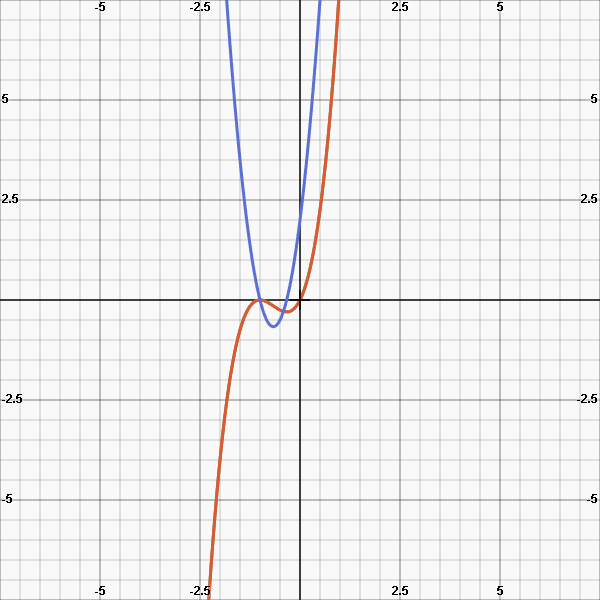
\includegraphics[width=0.7\textwidth]{FirstandSecondDegreeSurfaceInteractions.png} % Replace with actual plot
    \caption{Degrees of Surface Interaction: D=0 (point at $2\pi$) represents stable orbit within the Radiation Source; D=1 (blue parabola) shows a particle breaking free but reabsorbed by the originating Radiation Source (positive region); D=2 (red escape trajectory) depicts a particle escaping toward a neighboring Radiation Source (negative region). The $x$-axis at $x=0$ marks the boundary between the two Radiation Sources, with the positive $y$-values representing the originating Radiation Source and the negative $y$-values the neighboring one.}
\end{figure}

\section{Earth as a Recursive Model}
Consider Earth:
\[
r_{\text{surface}} = 6363 \text{ km}, \quad g_{\text{surface}} \approx 9.81 \text{ m/s}^2.
\]
At the center ($m_1 = 0$), Gravitation is $100\%$. As $r$ increases, stored Gravitation converts to extended Radiation. At the Surface:
\[
G = R \quad \Rightarrow \quad E = G \cdot R.
\]
Here, Radiation equals Gravitation, resulting in the known acceleration due to gravity.

\section{Classical and Recursive Agreement}
For two separate Radiation Sources (e.g., Earth and Moon), the model reduces to classical Newtonian gravitation. The recursive model preserves this classical relationship while providing internal mass distribution analysis.

\section{Conclusion}
The recursive gravitation model maintains Newtonian accuracy between distinct bodies while extending its applicability to single-body systems. By addressing Degrees of Surface Interaction, it offers new perspectives on mass-energy interactions, radiation emission, and gravitational equilibrium.

\end{document}
